% Báo cáo tiếng Việt giải thích chi tiết thiết kế thí nghiệm và kết quả.
% Biên dịch: tectonic baocao_vi.tex  (XeTeX, cần font TeX Gyre có sẵn trong bundle)
\documentclass[11pt]{article}
\usepackage[margin=1in]{geometry}
\usepackage{fontspec}
\setmainfont{texgyretermes}[Extension=.otf,UprightFont=*-regular,BoldFont=*-bold,
  ItalicFont=*-italic,BoldItalicFont=*-bolditalic]
\setsansfont{texgyreheros}[Extension=.otf,UprightFont=*-regular,BoldFont=*-bold,
  ItalicFont=*-italic,BoldItalicFont=*-bolditalic]
\setmonofont{texgyrecursor}[Extension=.otf,UprightFont=*-regular,BoldFont=*-bold,
  ItalicFont=*-italic,BoldItalicFont=*-bolditalic,Scale=0.95]
\usepackage{amsmath,amssymb,amsthm,mathtools}
\usepackage{booktabs,multirow,array,tabularx}
\usepackage{xcolor}
\usepackage{tikz}
\usetikzlibrary{arrows.meta,positioning,calc,shapes.geometric}
\usepackage{pgfplots}
\pgfplotsset{compat=1.17}
\usepackage[most]{tcolorbox}
\usepackage{enumitem}
\usepackage{caption}
\usepackage[hidelinks]{hyperref}

\renewcommand{\contentsname}{Mục lục}
\renewcommand{\tablename}{Bảng}
\renewcommand{\figurename}{Hình}
\renewcommand{\abstractname}{Tóm tắt}
\renewcommand{\refname}{Tài liệu tham khảo}
\captionsetup{font=small,labelfont=bf}

\newtheorem{menhde}{Mệnh đề}
\newtheorem{giadinh}{Giả định}

\definecolor{xanh}{HTML}{2E6BD9}
\definecolor{doxam}{HTML}{B42318}
\definecolor{luc}{HTML}{1F7A4D}
\definecolor{cam}{HTML}{D9822B}
\definecolor{mau1}{HTML}{2E6BD9}
\definecolor{mau2}{HTML}{D9822B}
\definecolor{mau3}{HTML}{1F7A4D}
\definecolor{xam}{HTML}{9AA5B1}

\newtcolorbox{vidu}[1][]{colback=xanh!4,colframe=xanh!60,fonttitle=\bfseries\small,
  title={Ví dụ#1},boxrule=0.5pt,arc=2pt,left=6pt,right=6pt,top=4pt,bottom=4pt}
\newtcolorbox{cachdoc}{colback=luc!5,colframe=luc!70,fonttitle=\bfseries\small,
  title={Cách đọc kết quả},boxrule=0.5pt,arc=2pt,left=6pt,right=6pt,top=4pt,bottom=4pt}
\newtcolorbox{thietke}{colback=cam!6,colframe=cam!80,fonttitle=\bfseries\small,
  title={Vì sao thiết kế như vậy},boxrule=0.5pt,arc=2pt,left=6pt,right=6pt,top=4pt,bottom=4pt}
\newtcolorbox{ketluan}{colback=black!4,colframe=black!60,fonttitle=\bfseries\small,
  title={Kết luận},boxrule=0.5pt,arc=2pt,left=6pt,right=6pt,top=4pt,bottom=4pt}

\newcommand{\dn}{\mathrm{do}_{\text{naive}}}
\newcommand{\dt}{\mathrm{do}_{\text{total}}}
\newcommand{\ci}[2]{{\scriptsize[#1,\,#2]}}

\setlength{\parskip}{3pt}

\title{\textbf{Read, Not Reasoned?}\\[4pt]
\large Báo cáo chi tiết bằng tiếng Việt: thiết kế thí nghiệm, phương pháp và kết quả}
\author{[Họ tên học viên] \quad·\quad GVHD: [Tên giáo sư hướng dẫn]}
\date{Bản đi kèm paper tiếng Anh \texttt{paper/main.pdf}}

\begin{document}
\maketitle

\begin{abstract}
Báo cáo này giải thích lại toàn bộ nghiên cứu ``Read, Not Reasoned?'' theo cách dễ theo dõi hơn
bản paper tiếng Anh. Câu hỏi trung tâm: khi một mô hình ngôn ngữ nhỏ (0.5B--7B tham số) viết
chain-of-thought (CoT) cho câu hỏi nhiều bước, đáp án cuối cùng có thật sự được \emph{suy ra} từ
chuỗi đó, hay mô hình chỉ \emph{đọc lại} chữ đã có sẵn trong chuỗi? Để trả lời, chúng tôi dựng
các phép thử mà \emph{đáp án đúng của chính phép thử} đã biết trước: biết bước nào cần thiết, biết
can thiệp nào lẽ ra không được làm đổi đáp án. Mỗi thí nghiệm được trình bày theo cùng một khung:
mục đích, thiết kế và lý do thiết kế, ví dụ, kết quả, cách đọc kết quả và kết luận.

Năm kết quả chẩn đoán: (R1) che một bước đơn lẻ bỏ sót suy luận kiểu bridge; (R2) đo
``necessity'' bằng resampling với baseline cố định bị lệch đúng bằng $1-r$; (R3) chuỗi được đọc
chứ không được suy luận, và mô hình $\le$3B chép cả đáp án sai mà nó tự giải được; (R4) distractor
làm hại CoT \emph{thông qua} chuỗi; (R5) vì vậy decoding ở bước đọc đáp án (HGCD) không giúp gì.
Phần decoding (round 9) cho thấy: lọc distractor bằng attention của mô hình không vượt
self-consistency trên MuSiQue, nhưng \textbf{đưa phép hợp thành ra ngoài mô hình} tăng accuracy
CLUTRR thêm 21--37 điểm so với self-consistency cùng compute, và ablation chứng minh mức tăng đến
từ chính bước hợp thành.
\end{abstract}

\tableofcontents
\newpage

% ==================================================================================
\section{Đọc nhanh: toàn bộ nghiên cứu trong hai trang}

\paragraph{Vấn đề.} CoT giúp mô hình trả lời tốt hơn, nhưng \emph{viết} ra một bước không có nghĩa
là \emph{dùng} bước đó. Nhiều nghiên cứu đã thử đo mức độ ``faithful'' của CoT bằng cách xoá hoặc
sửa một bước rồi xem đáp án có đổi không. Điểm yếu chung là thiếu \textbf{ground truth}: không ai
biết bước nào thật sự cần thiết, nên không thể kiểm chứng phương pháp đo nào đúng, chỉ có thể so
các phương pháp với nhau.

\paragraph{Cách tiếp cận.} Chúng tôi tạo ground truth theo ba cách:
\begin{enumerate}[leftmargin=*,itemsep=1pt]
\item \textbf{Chuỗi gold}: viết sẵn chuỗi đúng từ đường đi gold của dữ liệu.
\item \textbf{Bước thừa} (redundant hop): chèn vào chuỗi một bước đúng sự thật nhưng không liên
  quan đến câu hỏi. Mức cần thiết thật của nó bằng 0.
\item \textbf{Can thiệp có hiệu ứng thật bằng 0}: đổi tên người, đổi thứ tự câu, thêm distractor.
  Về mặt logic, đáp án đúng không thay đổi.
\end{enumerate}
Ngoài ra, chúng tôi làm \textbf{mediation chính xác}: tự đặt chuỗi vào mô hình, nhờ đó quan sát
được hiệu ứng trực tiếp và gián tiếp trên từng câu hỏi thay vì phải ước lượng.

\begin{table}[h]
\centering\small
\caption{Tóm tắt các kết quả.}
\label{tab:tomtat}
\begin{tabularx}{\linewidth}{@{}l>{\raggedright\arraybackslash}X>{\raggedright\arraybackslash}X@{}}
\toprule
\# & Kết quả & Giải thích một câu \\
\midrule
R1 & Che một bước đơn lẻ ($\dn$) bỏ sót bước cần thiết; che kèm các bước phụ thuộc ($\dt$) thì đúng
   & Bước sau đã chép lại kết quả của bước trước, nên che bước trước một mình không mất thông tin \\
R2 & Resampling với baseline cố định bị lệch đúng bằng $1-r$
   & Mô hình chỉ tự viết tiếp đúng 22--44\% số lần, nên bước nào cũng bị coi là ``cần thiết'' \\
R3 & \textbf{Chuỗi được đọc, không được suy luận}
   & Đáp án chỉ phụ thuộc vào chuỗi khi đáp án được viết sẵn trong chuỗi; mô hình $\le$3B chép cả
     đáp án sai dù tự giải được \\
R4 & Distractor làm hại CoT \emph{thông qua} chuỗi
   & Giữ nguyên chuỗi cũ thì distractor gần như không còn tác hại \\
R5 & Decoding ở bước đọc đáp án (HGCD) không giúp
   & Không thể khuếch đại một sự phụ thuộc không tồn tại \\
\midrule
D1 & MuSiQue: lọc distractor trước khi sinh chuỗi: \textcolor{doxam}{\textbf{thất bại}}
   & Attention của mô hình $\le$3B chọn chưa đủ chính xác; self-consistency vẫn tốt nhất \\
D2 & CLUTRR: mô hình chỉ trích fact, bảng luật hợp thành: \textcolor{luc}{\textbf{thành công}}
   & +21 đến +37 điểm (chuỗi ngắn); +24 điểm (chuỗi dài, 7B) so với SC cùng compute \\
D3 & Ablation: cùng fact, đổi bên hợp thành
   & LLM tự hợp thành $\approx$ CoT; bảng luật tốt hơn 13--35 điểm, nên nút thắt là bước hợp thành \\
\bottomrule
\end{tabularx}
\end{table}

\begin{ketluan}
Mô hình nhỏ \emph{đọc} chuỗi chứ không \emph{suy luận qua} chuỗi. Vì vậy chỉnh cách chọn token ở
bước đọc đáp án không giúp được gì, còn đưa bước suy luận ra ngoài mô hình thì giúp rất nhiều.
\end{ketluan}

\paragraph{Mạch lập luận.} Các thí nghiệm không rời rạc mà nối thành một chuỗi:
R1--R2 xây dựng \emph{thước đo đúng} (và chỉ ra hai thước đo sai phổ biến) $\Rightarrow$
R3--R4 dùng thước đo đó để \emph{chẩn đoán} chỗ hỏng $\Rightarrow$
R5 và D1 kiểm tra các phương pháp decoding mà chẩn đoán dự đoán sẽ thất bại $\Rightarrow$
D2--D3 kiểm tra phương pháp mà chẩn đoán dự đoán sẽ thành công, và chứng minh cơ chế bằng ablation.

% ==================================================================================
\section{Bài toán và mô hình nhân quả}

\subsection{Hai loại câu hỏi nhiều bước}

Toàn bộ nghiên cứu dựa trên việc so sánh hai loại bài toán có cấu trúc khác nhau.

\begin{vidu}[: bridge chain (MuSiQue)]
\textbf{Câu hỏi:} Vợ của đạo diễn phim X là ai?\\
\texttt{Hop 1: Đạo diễn phim X là ... => Y}\\
\texttt{Hop 2: Vợ của Y là ... => Z}\\
\textbf{Đáp án:} Z. Mỗi bước tìm ra một thực thể, bước sau dùng thực thể đó. Đáp án \emph{được
viết ra} ở bước cuối, nên muốn trả lời chỉ cần đọc bước cuối.
\end{vidu}

\begin{vidu}[: compositional chain (CLUTRR)]
\textbf{Câu chuyện:} Anna đưa con trai Ben đi sở thú. Ben và chị gái Clara nướng bánh.
\textbf{Hỏi:} Clara là gì của Anna?\\
\texttt{Hop 1: Ben là con trai (son) của Anna.}\\
\texttt{Hop 2: Clara là chị/em gái (sister) của Ben.}\\
\textbf{Đáp án:} Clara là \emph{con gái} (daughter) của Anna, vì son $\circ$ sister $=$ daughter.
Chữ ``daughter'' \emph{không xuất hiện} trong chuỗi. Muốn trả lời đúng, mô hình phải tự tính phép
hợp thành.
\end{vidu}

Đây là chìa khoá của nghiên cứu. Nếu mô hình trả lời đúng ở cả hai loại nhưng chỉ phụ thuộc vào
chuỗi ở loại bridge, thì nó đang \emph{đọc} chứ không \emph{suy luận}.

\subsection{Structural causal model (SCM) của bài toán}

Các biến gồm: câu hỏi $Q$; ngữ cảnh $P$ gồm các đoạn đúng $P_{\text{sup}}$ và distractor
$P_{\text{dist}}$; các bước $H_1,\dots,H_k$; đáp án $A$. Mỗi bước có dạng
\texttt{Hop $i$: <nội dung> => <kết quả>}.

\begin{figure}[h]
\centering
\begin{tikzpicture}[node distance=1.1cm and 1.25cm, every node/.style={font=\small},
  v/.style={draw,circle,minimum size=7mm,inner sep=0pt}, ar/.style={-{Stealth[length=2mm]}}]
\node[v] (q) {$Q$};
\node[v,right=of q] (h1) {$H_1$};
\node[v,right=of h1] (h2) {$H_2$};
\node[v,right=of h2] (h3) {$H_3$};
\node[v,right=of h3] (a) {$A$};
\node[v,above=of h1] (p1) {$P_1$};
\node[v,above=of h2] (p2) {$P_2$};
\node[v,above=of h3] (p3) {$P_3$};
\node[v,above=of a,draw=red!70,text=red!70] (pd) {$P_{\!d}$};
\draw[ar] (q)--(h1); \draw[ar] (h1)--(h2); \draw[ar] (h2)--(h3); \draw[ar] (h3)--(a);
\draw[ar] (p1)--(h1); \draw[ar] (p2)--(h2); \draw[ar] (p3)--(h3);
\draw[ar,dashed,blue!70] (h1) to[bend right=30] (a);
\draw[ar,dashed,blue!70] (h2) to[bend right=22] (a);
\draw[ar,dotted,red!70] (pd)--(a);
\draw[ar,dotted,gray] (q) to[bend right=40] node[below,font=\scriptsize]{đường tắt (shortcut)} (a);
\end{tikzpicture}
\caption{SCM của bài toán. Nét liền: chuỗi bridge. Nét đứt xanh: các cạnh thêm của chuỗi
compositional (mọi bước đều góp vào đáp án). Chấm đỏ: đường ``lậu'' từ distractor tới đáp án,
mô hình có thể dùng nhưng đồ thị bài toán cấm. Chấm xám: đường tắt dựa vào tri thức có sẵn của
mô hình.}
\label{fig:scm}
\end{figure}

\begin{thietke}
Chúng tôi \emph{không} giả định mô hình ngôn ngữ \emph{là} một SCM. SCM chỉ mô tả bài toán và cung
cấp ground truth: bước nào cần thiết, can thiệp nào lẽ ra không làm đổi đáp án. Mô hình được coi
là một ``người đọc'' (reader) tất định: cho cùng input thì cho cùng phân phối đáp án. Vì vậy, khi
ta sửa chữ trong chuỗi rồi đưa vào mô hình, đó là một \emph{can thiệp chính xác lên input của
người đọc}, và thay đổi xác suất đáp án là hiệu ứng \emph{quan sát được}, không phải ước lượng.
\end{thietke}

\subsection{Đồ thị suy luận (DRG) và các kiểu can thiệp}

\paragraph{DRG (Directed Reasoning Graph).} Từ một chuỗi, nối $i\to j$ ($i<j$) nếu kết quả của
bước $i$ được nhắc lại trong nội dung bước $j$. Các bước ``tổ tiên'' của bước cuối trong DRG là
các bước liên quan tới đáp án; những bước còn lại không có đường đi tới đáp án.

\paragraph{Các kiểu can thiệp lên bước $j$:}
\begin{itemize}[leftmargin=*,itemsep=1pt]
\item $\dn(j)$: thay bước $j$ bằng \texttt{[MASKED]}, giữ nguyên mọi bước khác.
\item $\dt(j)$: che bước $j$ \emph{và} mọi chỗ các bước con cháu trong DRG nhắc lại kết quả của
  $j$ (và kết quả của chính các bước con cháu đó). Đây là xấp xỉ tất định của
  $\mathrm{do}(H_j=\bot)$: nếu $H_j$ không được biết thì mọi thứ suy ra từ nó cũng không được biết.
\item \textbf{Placebo}: viết lại bước $j$ bằng câu chữ khác nhưng giữ nguyên thực thể và quan hệ.
  Hiệu ứng lẽ ra $\approx 0$.
\item \textbf{Mask-marker}: chèn token \texttt{[MASKED]} vào bước $j$ nhưng \emph{giữ nguyên} nội
  dung. Đo xem bản thân token mask có gây nhiễu không.
\item \textbf{Marker-tree} (volume-matched): chèn cùng \emph{số lượng} token mask như $\dt$ vào
  bước $j$ và các bước con cháu, nhưng giữ nội dung. Kiểm tra xem hiệu ứng lớn của $\dt$ có phải
  chỉ vì nó che nhiều chữ hơn không.
\end{itemize}

Đại lượng đo chính: $\Delta_j = p(\text{gold}\mid\text{chuỗi gốc}) - p(\text{gold}\mid
\text{chuỗi bị can thiệp})$, tính bằng điểm phần trăm. Trong đó $p(\text{gold})$ là xác suất mô hình
gán cho đáp án đúng, chuẩn hoá trên tập ứng viên.

\begin{vidu}[: hai kiểu che trên chuỗi bridge]
Chuỗi gốc: \texttt{Hop 1: Đạo diễn phim X là ... => Y. Hop 2: Vợ của Y là ... => Z.}\\
$\dn(1)$: \texttt{Hop 1: [MASKED]. Hop 2: Vợ của \textbf{Y} là ... => Z.} Chữ Y vẫn còn ở Hop 2.\\
$\dt(1)$: \texttt{Hop 1: [MASKED]. Hop 2: Vợ của \textbf{[MASKED]} là ... => [MASKED].}
\end{vidu}

% ==================================================================================
\section{Dữ liệu, mô hình và thống kê}

\begin{table}[h]
\centering\small
\caption{Thiết lập chung.}
\begin{tabularx}{\linewidth}{@{}l>{\raggedright\arraybackslash}X@{}}
\toprule
Mục & Chi tiết \\
\midrule
CLUTRR & Task \texttt{gen\_train234\_test2to10}, chỉ giữ câu chuyện ``sạch'' có một đường đi đơn
  (11.708 train / 635 test). Round 9 dùng thêm task \texttt{gen\_train23\_test2to10} làm dữ liệu
  \emph{chưa từng dùng} trong lúc phát triển phương pháp. \\
MuSiQue-Ans & Câu hỏi Wikipedia thật, có gold decomposition. Ngữ cảnh gồm các đoạn đúng và 4
  distractor (8 distractor với can thiệp \texttt{dist8}). MuSiQue được xây dựng để chống trả lời
  bằng đường tắt một bước. \\
Mô hình & Qwen2.5-0.5B/1.5B/3B/7B-Instruct và SmolLM2-1.7B-Instruct (hai họ mô hình); fp16,
  greedy decoding. \\
Phần cứng & Kaggle T4 16GB (7B chia trên 2 T4). Không fine-tune. \\
Thống kê & 95\% CI bằng bootstrap 2.000 lần (resample theo câu hỏi, không theo bước); so sánh cặp
  bằng paired bootstrap và McNemar. \\
\bottomrule
\end{tabularx}
\end{table}

\paragraph{Một số thuật ngữ thống kê.}
\begin{itemize}[leftmargin=*,itemsep=1pt]
\item \textbf{AUC}: khả năng phân biệt bước cần thiết với bước thừa dựa trên điểm số của một
  phương pháp đo. 0.5 nghĩa là đoán mò, 1.0 là phân biệt hoàn hảo.
\item \textbf{PS $=1$}: câu hỏi mà mô hình tự giải đúng từ chuỗi gold.
\item \textbf{TE / NDE / TIE}: hiệu ứng tổng / trực tiếp (không đi qua chuỗi) / gián tiếp (đi qua
  chuỗi). Xem \S\ref{sec:r4}.
\item \textbf{SC} (self-consistency): sinh nhiều chuỗi rồi bỏ phiếu đa số. SC$_n$ là $n$ mẫu.
\item \textbf{Cùng compute}: baseline được cấp ngân sách sinh không ít hơn phương pháp đang so sánh.
\item \textbf{Go/no-go đăng ký trước}: ngưỡng thành công được ghi vào \texttt{REVIEW.md}
  \emph{trước} khi chạy GPU. Ở round 9, ngưỡng là vượt baseline tốt nhất ít nhất 2 điểm với 95\%
  CI của paired bootstrap $>0$.
\end{itemize}

% ==================================================================================
\section{Phần A: xây dựng thước đo đúng}

\subsection{Thiết kế chung: estimator benchmark}

\begin{thietke}
Để biết một phương pháp đo ``mức cần thiết của bước'' có đúng không, cần dữ liệu mà ta \emph{biết
trước} bước nào cần thiết. Với mỗi chuỗi gold, chúng tôi chèn \textbf{một bước đúng sự thật nhưng
không nằm trên đường suy luận} (necessity $=0$). Một phương pháp đo tốt phải cho điểm cao với các
bước gold và điểm $\approx 0$ với bước chèn. Chất lượng được tóm tắt bằng AUC.

Bước chèn cũng bị che \emph{y hệt} các bước khác. Vì vậy, nếu bản thân token mask gây nhiễu, nhiễu
đó sẽ xuất hiện trên bước chèn và làm giảm AUC. Thiết kế này tự kiểm soát artifact của mask.
\end{thietke}

Mỗi mô hình được đo trên 180 chuỗi CLUTRR và 150 chuỗi MuSiQue, tổng khoảng 2.800 bước được chấm
điểm. Với Qwen-7B dùng 120 và 100 chuỗi, không chạy resampling vì giới hạn GPU. Các phương pháp
được so sánh:
\begin{enumerate}[leftmargin=*,itemsep=1pt]
\item $\dn$: che một bước.
\item $\dt$: che bước và các bước con cháu.
\item Counterfactual: thay kết quả của bước bằng một thực thể khác, có hoặc không lan truyền sang
  các bước sau. Cách này không dùng token mask.
\item Resampling với baseline cố định và với baseline resample ($K=2$ mẫu mỗi nhánh).
\item Ba control: placebo, mask-marker, marker-tree.
\end{enumerate}
Ngoài $p(\text{gold})$ chuẩn hoá trên tập ứng viên, chúng tôi còn đo trên raw log-probability để
chắc chắn kết luận không phụ thuộc vào cách chọn tập ứng viên.

% ----------------------------------------------------------------------------------
\subsection{R1: che một bước đơn lẻ bỏ sót suy luận kiểu bridge}

\paragraph{Mục đích.} Kiểm tra phương pháp phổ biến nhất trong literature, ``xoá một bước xem đáp
án có đổi không'', có đo đúng mức cần thiết không.

\paragraph{Dự đoán lý thuyết.}
\begin{giadinh}[Người đọc Markov trên chuỗi bridge]
Trên chuỗi bridge, nếu bước $j+1$ nhắc lại kết quả của bước $j$, thì xác suất đáp án chỉ phụ thuộc
vào $h_{1:j}$ thông qua $h_{j+1:k}$.
\end{giadinh}
\begin{menhde}
$\Delta^{\text{naive}}_j$ đúng bằng \emph{controlled direct effect} của $H_j$ lên $A$ khi các bước
sau được giữ cố định. Dưới Giả định 1, $\Delta^{\text{naive}}_j=0$ với mọi bước không phải bước
cuối trên chuỗi bridge, trong khi $\Delta^{\text{total}}_j$ không bị ràng buộc bằng 0.
\end{menhde}
Nói đơn giản: che Hop 1 nhưng Hop 2 vẫn ghi ``Y'' thì mô hình không mất thông tin gì, nên $\dn$
luôn báo ``không cần thiết'', \emph{kể cả khi Hop 1 thật sự cần thiết}. Đây là một đồng nhất thức,
không phải nhiễu thống kê.

\begin{figure}[h]
\centering
\begin{tikzpicture}
\begin{axis}[ybar, width=0.92\linewidth, height=5.2cm, bar width=9pt, ymin=-10, ymax=80,
  symbolic x coords={Q-0.5B,Q-1.5B,Smol-1.7B,Q-3B,Q-7B}, xtick=data,
  ylabel={$\Delta p(\text{gold})$ (điểm)}, legend style={at={(0.5,1.03)},anchor=south,legend columns=4,font=\small,draw=none},
  nodes near coords, every node near coord/.append style={font=\tiny}, enlarge x limits=0.12,
  ymajorgrids, grid style={black!10}]
\addplot[fill=mau1,draw=none] coordinates {(Q-0.5B,56.7)(Q-1.5B,56.9)(Smol-1.7B,66.8)(Q-3B,49.1)(Q-7B,41.3)};
\addplot[fill=mau2,draw=none] coordinates {(Q-0.5B,-2.4)(Q-1.5B,0.6)(Smol-1.7B,-3.9)(Q-3B,0.5)(Q-7B,6.5)};
\addplot[fill=xam,draw=none] coordinates {(Q-0.5B,7.3)(Q-1.5B,0.0)(Smol-1.7B,2.3)(Q-3B,-0.3)(Q-7B,5.7)};
\addplot[fill=mau3,draw=none] coordinates {(Q-0.5B,-4.5)(Q-1.5B,0.4)(Smol-1.7B,-1.2)(Q-3B,-1.5)(Q-7B,-1.6)};
\legend{$\dt$ (bước gold), $\dn$ (bước gold), marker-tree (control), $\dt$ (bước thừa)}
\end{axis}
\end{tikzpicture}
\caption{R1 trên MuSiQue: tác động lên $p(\text{gold})$ khi che một bước không phải bước cuối.}
\label{fig:r1}
\end{figure}

\begin{table}[h]
\centering\small
\caption{AUC phân biệt bước cần thiết với bước thừa (0.5 = đoán mò).}
\label{tab:auc}
\begin{tabular}{llccccc}
\toprule
Dữ liệu & Phương pháp & Q-0.5B & Q-1.5B & Smol-1.7B & Q-3B & Q-7B \\
\midrule
MuSiQue & $\dt$ & 0.94 & 0.98 & 0.98 & 0.97 & 0.86 \\
        & $\dn$ & 0.72 & 0.82 & 0.66 & 0.76 & 0.71 \\
        & counterfactual, lan truyền & 0.94 & 0.99 & 0.98 & 0.97 & 0.87 \\
        & $\dt$, raw log-prob & 0.99 & 0.99 & 1.00 & 0.98 & 0.88 \\
        & placebo (control) & 0.51 & 0.48 & 0.50 & 0.47 & 0.54 \\
\midrule
CLUTRR + copy & $\dt$ & 1.00 & 1.00 & 1.00 & 0.99 & 0.95 \\
        & $\dn$ & 0.64 & 0.67 & 0.65 & 0.70 & 0.72 \\
        & marker-tree (control) & 0.95 & 0.61 & 0.82 & 0.78 & 0.64 \\
\bottomrule
\end{tabular}
\end{table}

\begin{cachdoc}
\begin{itemize}[leftmargin=*,itemsep=1pt]
\item $\dt$ làm $p(\text{gold})$ giảm 41--67 điểm; $\dn$ gần như không đổi gì ($-3.9$ đến $+6.5$),
  đúng như mệnh đề dự đoán (Hình~\ref{fig:r1}).
\item Bước thừa bị che bằng $\dt$ gần như không ảnh hưởng ($\approx 0$). Vậy $\dt$ không ``che
  bừa'': nó chỉ tác động lên bước thật sự cần thiết.
\item Control marker-tree (cùng số token mask nhưng giữ nội dung) chỉ gây 0--7 điểm. Hiệu ứng lớn
  của $\dt$ \emph{không phải} do che nhiều chữ. Placebo ở mức đoán mò, đúng như phải thế.
\item Hai cách đo không dùng mask hoặc không cần tập ứng viên (counterfactual, raw log-prob) cho
  kết luận giống hệt (Bảng~\ref{tab:auc}).
\item Ngoại lệ trung thực: ở Q-0.5B, marker-tree trên CLUTRR+copy vẫn có AUC 0.95, tức control
  dựa trên mask chưa hoàn toàn ``trơ'' ở mô hình nhỏ nhất. Điều này được ghi trong phần hạn chế.
\end{itemize}
\end{cachdoc}

\begin{ketluan}
Muốn đo một bước có cần thiết không, phải can thiệp cả các bước phụ thuộc vào nó. Phương pháp
``xoá một bước'' đánh giá thấp có hệ thống mức cần thiết của các bước trung gian.
\end{ketluan}

% ----------------------------------------------------------------------------------
\subsection{R2: resampling với baseline cố định bị lệch $1-r$}

\paragraph{Mục đích.} Kiểm tra cách đo thứ hai trong literature: làm hỏng một bước, cho mô hình
\emph{tự viết tiếp phần còn lại}, rồi xem tỷ lệ trả lời đúng giảm bao nhiêu (``probability of
necessity'').

\paragraph{Vấn đề.} Nhiều phương pháp so kết quả sau khi làm hỏng với chuỗi gold gốc, vốn luôn
đúng (baseline cố định). Nhưng ngay cả khi \emph{không} làm hỏng gì, mô hình tự viết tiếp cũng chỉ
đúng với tỷ lệ $r<1$. Phần sai do mô hình viết tiếp kém ($1-r$) bị tính nhầm thành ``do bước bị
làm hỏng''.

\begin{menhde}
Gọi $q_j$ là xác suất đúng khi bước $j$ bị làm hỏng rồi viết tiếp, $r_j$ là xác suất đúng khi giữ
bước $j$ rồi viết tiếp. Trên các câu mà chuỗi gốc cho đáp án đúng, ước lượng với baseline cố định
bằng $1-q_j=(r_j-q_j)+(1-r_j)$: hiệu ứng thật cộng một độ lệch $1-r_j\ge 0$ \emph{không phụ thuộc}
vào việc bước $j$ có cần thiết hay không. Với bước thừa ($r_j=q_j$), nó trả về $1-r_j$ thay vì 0.
\end{menhde}

\begin{vidu}[: con số cụ thể]
Giả sử mô hình tự viết tiếp đúng chỉ 30\% số lần ($r=0.3$). Khi đó \emph{mọi} bước, kể cả bước
hoàn toàn không liên quan, đều bị chấm ``cần thiết'' khoảng 70 điểm. Cách sửa: so với một baseline
\emph{cũng được resample} (giữ bước $j$, cho viết tiếp), tức là đo $r_j-q_j$.
\end{vidu}

\begin{table}[h]
\centering\small
\caption{R2 trên MuSiQue: điểm ``cần thiết'' (điểm phần trăm).}
\label{tab:r2}
\begin{tabular}{lcccc}
\toprule
 & Q-0.5B & Q-1.5B & Smol-1.7B & Q-3B \\
\midrule
Baseline cố định: bước cần thiết & 79.0 & 75.7 & 68.9 & 61.5 \\
Baseline cố định: \textbf{bước thừa} & \textbf{78.0} & \textbf{76.3} & \textbf{72.7} & \textbf{56.3} \\
Baseline resample: bước cần thiết & 3.5 & 6.4 & $-0.2$ & 11.3 \\
Baseline resample: bước thừa & 1.7 & $-0.3$ & 3.3 & 4.3 \\
\midrule
AUC, baseline cố định & 0.51 & 0.52 & 0.51 & 0.55 \\
AUC, baseline resample & 0.65 & 0.67 & 0.61 & 0.64 \\
\bottomrule
\end{tabular}
\end{table}

\begin{cachdoc}
\begin{itemize}[leftmargin=*,itemsep=1pt]
\item Với baseline cố định, bước thừa bị chấm ``cần thiết'' 56--78 điểm, ngang bước thật sự cần
  thiết; AUC 0.51--0.55, tức đoán mò. Con số 56--78 chính là $1-r$: mô hình chỉ tự viết tiếp đúng
  22--44\% số lần.
\item Với baseline resample, bước thừa về $\approx 0$ đúng như mệnh đề, AUC tăng lên 0.61--0.67.
\item Bước cần thiết dưới resampling cũng chỉ 0--11 điểm, vì mô hình \emph{tự suy lại} bước bị hỏng
  từ ngữ cảnh. Resampling đo ``bước này có \emph{khôi phục được} không'' (recoverability), còn
  $\dt$ đo ``bước được viết ra có \emph{được dùng} không'' (use). Đây là hai câu hỏi khác nhau.
\end{itemize}
\end{cachdoc}

\begin{ketluan}
Một số phương pháp đo step necessity đã công bố cho ra con số chủ yếu phản ánh việc mô hình viết
tiếp kém, chứ không phản ánh tầm quan trọng của bước. Lemma nhận dạng của các nghiên cứu này ngầm
giả định $r=1$; R2 định lượng chuyện gì xảy ra khi giả định đó sai.
\end{ketluan}

% ==================================================================================
\section{Phần B: chẩn đoán}

\subsection{R3: chuỗi được đọc, không được suy luận}
\label{sec:r3}

\paragraph{Mục đích.} Trên CLUTRR, đáp án phải được \emph{tính} từ các bước và không xuất hiện
trong chuỗi. Nếu mô hình thật sự suy luận qua chuỗi, che một bước quan hệ phải làm đáp án thay đổi
nhiều. R3 gồm ba thí nghiệm nối tiếp nhau, mỗi thí nghiệm trả lời một câu hỏi mà thí nghiệm trước
để ngỏ.

\paragraph{Thí nghiệm 3a: che bước trên CLUTRR thường.} Dùng $\dt$ như R1, nhưng trên chuỗi
compositional.

\paragraph{Thí nghiệm 3b: một can thiệp nhị phân ``bật'' sự phụ thuộc ($T_{\text{copy}}$).} Giữ
nguyên mọi thứ, chỉ thêm \emph{một} bước cuối viết sẵn đáp án (``\dots vậy Clara là con gái của
Anna''). $T_{\text{copy}}\in\{0,1\}$ là biến can thiệp nhị phân.

\begin{thietke}
$T_{\text{copy}}$ biến chuỗi compositional thành chuỗi ``có chữ để chép'' mà không đổi gì khác:
cùng câu chuyện, cùng các bước quan hệ, cùng đáp án. Nếu sự phụ thuộc vào các bước quan hệ chỉ
xuất hiện khi $T_{\text{copy}}=1$, thì nguyên nhân là \emph{có đáp án viết sẵn}, không phải do
cấu trúc bài toán hay độ dài chuỗi.
\end{thietke}

\begin{figure}[h]
\centering
\begin{tikzpicture}
\begin{axis}[ybar, width=0.92\linewidth, height=5cm, bar width=11pt, ymin=-5, ymax=85,
  symbolic x coords={Q-0.5B,Q-1.5B,Smol-1.7B,Q-3B,Q-7B}, xtick=data,
  ylabel={$\Delta p(\text{gold})$ (điểm)}, legend style={at={(0.5,1.03)},anchor=south,legend columns=3,font=\small,draw=none},
  nodes near coords, every node near coord/.append style={font=\tiny}, enlarge x limits=0.12,
  ymajorgrids, grid style={black!10}]
\addplot[fill=xam,draw=none] coordinates {(Q-0.5B,0.1)(Q-1.5B,-1.5)(Smol-1.7B,1.8)(Q-3B,7.3)(Q-7B,1.3)};
\addplot[fill=mau1,draw=none] coordinates {(Q-0.5B,60.8)(Q-1.5B,76.1)(Smol-1.7B,69.5)(Q-3B,77.0)(Q-7B,51.9)};
\addplot[fill=mau2,draw=none] coordinates {(Q-0.5B,1.3)(Q-1.5B,1.3)(Smol-1.7B,1.0)(Q-3B,1.7)(Q-7B,0.9)};
\legend{CLUTRR thường: $\dt$, CLUTRR + copy: $\dt$, CLUTRR + copy: $\dn$}
\end{axis}
\end{tikzpicture}
\caption{R3: tác động của việc che một bước quan hệ (không phải bước cuối). Chỉ khi đáp án được
viết sẵn trong chuỗi, các bước mới có tác dụng.}
\label{fig:r3}
\end{figure}

\paragraph{Kết quả 3a và 3b.} Che hẳn một bước quan hệ trên CLUTRR thường hầu như không làm đáp án
thay đổi: $-1.5$ đến $+1.8$ điểm đến 1.7B, $7.3$ \ci{3.8}{11.0} ở 3B và $1.3$ \ci{-3.4}{6.0} ở 7B.
AUC trên CLUTRR chỉ 0.50--0.63, gần đoán mò. Thêm một bước viết sẵn đáp án thì các bước quan hệ
bỗng có hiệu ứng 52--77 điểm, giống hệt MuSiQue (Hình~\ref{fig:r3}).

\paragraph{Thí nghiệm 3c: ``không biết tính'' hay ``không thèm dùng chuỗi''?
($T_{\text{copy-wrong}}$).} Kết quả 3a có hai cách giải thích: (i) mô hình không biết tính phép hợp
thành nên đành chép, hoặc (ii) mô hình biết tính nhưng ưu tiên chép. Để tách hai khả năng, thêm một
bước cuối viết \textbf{đáp án sai} (``\dots vậy Clara là cháu gái của Anna''), mâu thuẫn với các
bước quan hệ. Đo tỷ lệ mô hình chép theo đáp án sai, và quan trọng nhất là trên các câu mà nó
\emph{tự giải đúng} từ chuỗi gold (PS $=1$).

\begin{table}[h]
\centering\small
\caption{R3c: tỷ lệ mô hình trả lời theo đáp án sai được viết sẵn (\%, 95\% CI).}
\label{tab:copywrong}
\begin{tabular}{lccc}
\toprule
Mô hình & Tự giải đúng (PS) & Chép sai, mọi câu & Chép sai, khi tự giải đúng \\
\midrule
Q-0.5B & 15.2 & 66.5 \ci{58.9}{74.1} & 70.8 \ci{54.2}{87.5} ($n=24$) \\
Q-1.5B & 17.1 & 58.2 \ci{50.6}{66.5} & 63.0 \ci{44.4}{81.5} ($n=27$) \\
Smol-1.7B & 26.6 & 56.3 \ci{48.1}{64.6} & 57.1 \ci{42.9}{71.4} ($n=42$) \\
Q-3B & 27.8 & 46.2 \ci{38.0}{54.4} & 47.7 \ci{34.1}{61.4} ($n=44$) \\
Q-7B & 33.1 & 22.9 \ci{16.1}{30.5} & \textbf{10.3} \ci{2.6}{20.5} ($n=39$) \\
\bottomrule
\end{tabular}
\end{table}

\begin{cachdoc}
\begin{itemize}[leftmargin=*,itemsep=1pt]
\item Đến 3B, mô hình chép đáp án sai \emph{thường xuyên như nhau} dù nó tự giải được câu đó hay
  không (cột 3 $\approx$ cột 4). Chữ viết sẵn trong chuỗi \emph{đè lên} lời giải của chính mô hình.
  Đây là bằng chứng cho cách giải thích (ii) ở mô hình nhỏ.
\item Ở 7B có một bước chuyển: mô hình chỉ chép sai 10\% trên các câu nó tự giải được, tức là nó
  đối chiếu đáp án viết sẵn với lời giải của mình và bác bỏ (veto) khi mâu thuẫn.
\item Nhưng ngay cả ở 7B, các bước quan hệ vẫn không có hiệu ứng đo được (3a: 1.3 điểm). Phép hợp
  thành của 7B không chạy \emph{qua} chuỗi đã viết.
\item Kiểm tra bổ sung: các chuỗi của chính mô hình chạm tới mọi thực thể trên đường gold cũng
  không làm accuracy của CoT cao hơn.
\end{itemize}
\end{cachdoc}

\begin{ketluan}
Ở mọi kích thước đã thử, sự phụ thuộc vào chuỗi đi theo thao tác mà mô hình làm được (chép một chuỗi
ký tự), chứ không đi theo suy luận mà chuỗi mô tả. Đây là kết quả trung tâm, và cũng là cơ sở cho
mọi thiết kế decoding ở Phần C.
\end{ketluan}

% ----------------------------------------------------------------------------------
\subsection{R4: distractor làm hại CoT thông qua chuỗi}
\label{sec:r4}

\paragraph{Mục đích.} Thêm distractor làm CoT sai nhiều hơn. Câu hỏi là tác hại đi theo đường nào:
trực tiếp từ distractor tới đáp án (chấm đỏ ở Hình~\ref{fig:scm}), hay qua việc mô hình
\emph{viết ra một chuỗi tệ hơn}?

\paragraph{Thiết kế: mediation chính xác.} Với mỗi câu hỏi, chạy ba lần:
\begin{enumerate}[leftmargin=*,itemsep=1pt]
\item $Y(0,M(0))$: input gốc, chuỗi gốc.
\item $Y(1,M(1))$: input có thêm 4 distractor (\texttt{dist8}), chuỗi được sinh lại.
\item $Y(1,M(0))$: input có distractor, nhưng \textbf{ép dùng lại chuỗi gốc}.
\end{enumerate}
Từ đó:
\[
\text{TE}=\mathbb{E}[Y(1,M(1))-Y(0,M(0))],\quad
\text{NDE}=\mathbb{E}[Y(1,M(0))-Y(0,M(0))],\quad
\text{TIE}=\text{TE}-\text{NDE}.
\]

\begin{thietke}
Trong mediation thông thường, $Y(1,M(0))$ là đại lượng ``phản thực xuyên thế giới'' (cross-world)
và không quan sát được, nên phải dựa vào các giả định mạnh. Ở đây mediator chính là \emph{văn bản}
chuỗi, nên ta có thể \emph{tự đặt} $M=M(0)$ dưới input mới. Nhờ vậy NDE và TIE được \emph{quan sát}
trên từng câu hỏi, không cần giả định.
\end{thietke}

\begin{figure}[h]
\centering
\begin{tikzpicture}
\begin{axis}[ybar, width=0.95\linewidth, height=5.2cm, bar width=10pt, ymin=-9, ymax=2,
  symbolic x coords={1.5B: Direct,1.5B: CoT,1.5B: CAD,3B: Direct,3B: CoT,3B: CAD}, xtick=data,
  x tick label style={font=\small},
  ylabel={Thay đổi EM (điểm)}, legend style={at={(0.5,1.03)},anchor=south,legend columns=2,font=\small,draw=none},
  nodes near coords, every node near coord/.append style={font=\tiny}, enlarge x limits=0.1,
  ymajorgrids, grid style={black!10}]
\addplot[fill=mau2,draw=none] coordinates {(1.5B: Direct,-4.6)(1.5B: CoT,1.0)(1.5B: CAD,-7.0)(3B: Direct,-3.8)(3B: CoT,-0.6)(3B: CAD,-5.0)};
\addplot[fill=mau1,draw=none] coordinates {(1.5B: Direct,-1.0)(1.5B: CoT,-3.6)(1.5B: CAD,-1.2)(3B: Direct,-2.0)(3B: CoT,-5.0)(3B: CAD,-2.4)};
\legend{NDE (trực tiếp, chuỗi cố định), TIE (gián tiếp, qua chuỗi)}
\end{axis}
\end{tikzpicture}
\caption{R4: phân rã tác hại của distractor (MuSiQue, \texttt{dist8}, $n=500$).}
\label{fig:r4}
\end{figure}

\begin{table}[h]
\centering\small
\caption{R4: mediation trên MuSiQue, $n=500$ (điểm EM, 95\% CI).}
\label{tab:r4}
\begin{tabular}{llccc}
\toprule
Mô hình & Phương pháp & TE & NDE (chuỗi cố định) & TIE (qua chuỗi) \\
\midrule
Qwen-1.5B & Direct (không CoT) & $-5.6$ \ci{-9.2}{-2.0} & $-4.6$ \ci{-7.4}{-1.6} & $-1.0$ \ci{-3.4}{1.6} \\
          & CoT & $-2.6$ \ci{-6.2}{1.2} & $\mathbf{+1.0}$ \ci{-0.8}{3.0} & $\mathbf{-3.6}$ \ci{-7.2}{0.0} \\
          & CAD & $-8.2$ \ci{-12.0}{-4.0} & $-7.0$ \ci{-10.2}{-3.6} & $-1.2$ \ci{-3.8}{1.6} \\
\midrule
Qwen-3B   & Direct (không CoT) & $-5.8$ \ci{-10.0}{-1.8} & $-3.8$ \ci{-7.4}{-0.2} & $-2.0$ \ci{-4.4}{0.4} \\
          & CoT & $-5.6$ \ci{-9.6}{-1.6} & $\mathbf{-0.6}$ \ci{-2.8}{1.8} & $\mathbf{-5.0}$ \ci{-8.8}{-1.0} \\
          & CAD & $-7.4$ \ci{-11.4}{-3.6} & $-5.0$ \ci{-8.6}{-1.6} & $-2.4$ \ci{-5.0}{0.2} \\
\bottomrule
\end{tabular}
\end{table}

\begin{cachdoc}
\begin{itemize}[leftmargin=*,itemsep=1pt]
\item Với CoT: nếu giữ nguyên chuỗi cũ thì distractor gần như vô hại (NDE $\approx 0$, CI chứa 0).
  Toàn bộ tác hại đến từ việc mô hình viết ra \emph{chuỗi khác} khi có distractor (TIE).
\item Với Direct và CAD thì ngược lại: tác hại chủ yếu là trực tiếp (NDE âm, có ý nghĩa).
\item Hệ quả cho decoding: CAD và các phương pháp ``tương phản ở bước đọc đáp án'' tác động lên
  đường trực tiếp, còn chỗ hỏng của CoT nằm ở đường gián tiếp. Chúng nhắm sai chỗ.
\item Độ lớn thật là 3--6 điểm. Pilot 120 câu trước đó báo khoảng $-10$ điểm do bị thổi phồng
  (winner's curse); bản $n=500$ đã sửa lại.
\item CoT \emph{không} dễ tổn thương hơn Direct về tổng thể: chênh lệch TE là $+3.0$
  \ci{-0.8}{6.8} và $+0.2$ \ci{-3.8}{4.2}, đều không có ý nghĩa. Claim cũ ``CoT dễ tổn thương
  hơn'' đã bị bỏ.
\end{itemize}
\end{cachdoc}

\begin{ketluan}
Distractor làm hại CoT bằng cách làm hỏng chuỗi được sinh ra, không phải bằng cách tác động trực
tiếp lên bước đọc đáp án. Muốn chống distractor phải can thiệp \emph{trước hoặc trong} lúc sinh
chuỗi.
\end{ketluan}

% ==================================================================================
\section{Phần C: decoding}

Phần này trả lời câu hỏi thực dụng: \emph{từ chẩn đoán trên, có cách decoding nào làm mô hình trả
lời đúng hơn không?} R3--R4 cho ra hai dự đoán:
\begin{enumerate}[leftmargin=*,itemsep=1pt]
\item Mọi phương pháp chỉnh xác suất \emph{ở bước đọc đáp án} sẽ không giúp, vì đáp án không phụ
  thuộc vào nội dung suy luận của chuỗi (R3) và tác hại của distractor không nằm ở đó (R4).
\item Một can thiệp \emph{thay thế} bước hợp thành (thứ mô hình không làm được) sẽ giúp.
\end{enumerate}

\subsection{R5: decoding ở bước đọc đáp án (HGCD), phương pháp ban đầu}

\paragraph{Thiết kế.} HGCD (Hop-Graph Causal Decoding) là phương pháp của đề xuất ban đầu. Ý tưởng:
khuếch đại phần đáp án ``do chuỗi gây ra''. Với các bước liên quan $\mathcal{R}(y)$ theo DRG, điểm
của mỗi đáp án $a$ là
\[
s_\alpha(a)=p(a\mid y)+\alpha\cdot\frac{1}{|\mathcal{R}(y)|}\sum_{j\in\mathcal{R}(y)}
\big[p(a\mid y)-p(a\mid\dt(j))\big],
\]
tức xác suất gốc cộng $\alpha$ lần hiệu ứng nhân quả trung bình của các bước liên quan. Các bước
thừa không bao giờ bị tương phản. $\alpha$ được chọn trên tập validation rồi cố định.

\begin{table}[h]
\centering\small
\caption{R5: accuracy (\%) của HGCD và calibration so với CoT.}
\label{tab:r5}
\begin{tabular}{lccc}
\toprule
 & CoT & HGCD & Calibration (content-free) \\
\midrule
CLUTRR · Qwen-1.5B & 18.1 & 18.1 & 23.9 \\
CLUTRR · SmolLM2-1.7B & 21.4 & 21.0 & 24.8 \\
MuSiQue · Qwen-1.5B & 20.8 & 22.5 & -- \\
MuSiQue · SmolLM2-1.7B & 15.0 & 15.8 & -- \\
\bottomrule
\end{tabular}
\end{table}

\begin{cachdoc}
\begin{itemize}[leftmargin=*,itemsep=1pt]
\item HGCD $=$ CoT ($|\Delta|\le 1.7$ điểm, mọi $p\ge 0.6$). Đúng như R3 dự đoán: không thể khuếch
  đại một sự phụ thuộc không tồn tại.
\item Calibration (Zhao và cộng sự, 2021) có tăng: $+5.9$ trên CLUTRR; $+4.0$ và $+5.4$ trên
  MuSiQue $n=500$. Nhưng nó không dùng thông tin gì từ chuỗi, và mong manh: đổi input ``rỗng''
  sang một câu trung tính thì SmolLM2 \emph{giảm} 5 điểm \ci{-10.1}{-0.4}. Kiểm tra sau đó cho thấy
  calibration $\approx$ sinh đáp án tự do (free generation), nên nó chỉ là baseline, không phải
  đóng góp phương pháp.
\item Giả định ``mixture reader'' đứng sau các mệnh đề về HGCD không được dữ liệu ủng hộ. Giả định
  này được ghi rõ trong appendix của paper là đã bị bác bỏ.
\end{itemize}
\end{cachdoc}

\subsection{Quy trình chung của round 9}

\begin{thietke}
Sau R5, mọi thí nghiệm decoding tuân theo một quy trình chống ``tự lừa mình'':
\begin{enumerate}[leftmargin=*,itemsep=1pt]
\item \textbf{Baseline mạnh}: so với cả CoT greedy và self-consistency \emph{cùng compute}, không
  chỉ với CoT. Nhiều paper decoding chỉ so với greedy; mức tăng của chúng thường biến mất trước SC.
\item \textbf{Đăng ký trước}: giả thuyết, tập dữ liệu, kiểm định chính và ngưỡng go/no-go được ghi
  vào \texttt{REVIEW.md} trước khi chạy.
\item \textbf{Phát hiện post hoc phải được xác nhận lại}: một cải tiến tìm thấy khi xem kết quả chỉ
  được chấp nhận sau khi chạy lại trên \emph{dữ liệu chưa dùng}, với giả thuyết đăng ký trước.
\end{enumerate}
\end{thietke}

% ----------------------------------------------------------------------------------
\subsection{D1: MuSiQue, lọc distractor trước khi sinh chuỗi}

\paragraph{Ý tưởng.} R4 cho thấy distractor hại CoT thông qua chuỗi. Vậy hãy bỏ distractor
\emph{trước} khi mô hình viết chuỗi, tức cắt đường $P_{\text{dist}}\to H$.

\paragraph{Các bộ chọn đoạn văn.}
\begin{itemize}[leftmargin=*,itemsep=1pt]
\item \textbf{Attn top-4}: đo attention của mô hình từ câu hỏi tới từng đoạn văn, hiệu chỉnh theo
  kiểu ICR (lấy attention với câu hỏi thật trừ đi attention với một câu hỏi rỗng ``N/A'' để khử
  thiên lệch vị trí), rồi chỉ giữ 4 đoạn cao nhất.
\item \textbf{Attn rerank}: giữ \emph{mọi} đoạn, chỉ sắp xếp lại theo điểm attention, nên không thể
  làm mất đoạn gold.
\item \textbf{Self-select}: hỏi chính mô hình đoạn nào liên quan.
\item \textbf{Gold only}: chỉ giữ các đoạn đúng. Đây là trần lý thuyết, không phải phương pháp.
\end{itemize}

\begin{table}[h]
\centering\small
\caption{D1: EM (\%) trên MuSiQue, $n=500$.}
\label{tab:d1}
\begin{tabular}{llcccccc}
\toprule
Distractor & Mô hình & CoT & SC$_5$ & Attn top-4 & Attn rerank & Self-select & Gold only \\
\midrule
4 & 1.5B & 24.8 & \textbf{28.4} & 23.6 & 23.0 & 13.2 & 34.8 \\
  & 3B   & 38.8 & \textbf{41.4} & 33.8 & 37.4 & 29.6 & 48.6 \\
\midrule
8 & 1.5B & 22.2 & \textbf{25.0} & 22.0 & 22.2 & 13.2 & 31.4 \\
  & 3B   & 31.6 & \textbf{35.6} & 27.4 & 33.6 & 24.8 & 45.6 \\
\bottomrule
\end{tabular}
\end{table}

\begin{cachdoc}
\begin{itemize}[leftmargin=*,itemsep=1pt]
\item Có chỗ để cải thiện: gold only cao hơn CoT 9--14 điểm.
\item Nhưng attention của mô hình $\le$3B chọn chưa đủ chính xác. Top-4 chỉ giữ đủ mọi đoạn gold ở
  77--86\% số câu (3B), và mất một đoạn gold thì accuracy giảm khoảng một nửa. Kết quả là top-4
  \emph{tệ hơn} CoT, rerank $\approx$ CoT, self-select tệ hẳn.
\item SC$_5$ vẫn tốt nhất. Kết luận: \textcolor{doxam}{\textbf{NO-GO}}.
\end{itemize}
\end{cachdoc}

\paragraph{Một bug đã được phát hiện và sửa.} Attention tính ở fp16 bị tràn số với Qwen-1.5B và
Qwen-7B (chia trên 2 GPU), khiến ``top-4'' thực chất luôn là 4 đoạn đầu tiên (500/500 câu). Lỗi
được phát hiện khi so lựa chọn của bộ chọn với một luật tầm thường (``giữ 4 đoạn đầu''). Bản sửa
tính lại bằng fp32 khi điểm không hữu hạn hoặc suy biến; 1.5B được chạy lại hoàn toàn (số trong
Bảng~\ref{tab:d1}), còn số liệu attention của 7B bị loại.

% ----------------------------------------------------------------------------------
\subsection{D2: CLUTRR, đưa phép hợp thành ra ngoài mô hình}

\paragraph{Ý tưởng.} R3 cho thấy mô hình \emph{đọc} tốt nhưng \emph{không hợp thành}. Vậy để mô
hình chỉ làm phần nó giỏi (đọc truyện, trích fact) và giao phép hợp thành cho một bảng luật. Về
mặt nhân quả, đây là \emph{thực thi} structural equation của đồ thị suy luận, thay vì để mô hình
bắt chước nó.

\begin{figure}[h]
\centering
\begin{tikzpicture}[font=\small, node distance=0.5cm,
  b/.style={draw,rounded corners=2pt,fill=#1,align=center,minimum height=1.5cm,text width=2.45cm,inner sep=3pt},
  ar/.style={-{Stealth[length=2mm]},thick}]
\node[b=xanh!10] (s) {Câu chuyện\\(văn bản)};
\node[b=cam!15,right=of s] (e) {\textbf{LLM} trích fact\\ và giới tính};
\node[b=black!5,right=of e] (g) {Đồ thị quan hệ\\ + cạnh nghịch đảo};
\node[b=black!5,right=of g] (p) {BFS: đường đi\\ nguồn $\to$ đích};
\node[b=luc!15,right=of p] (r) {\textbf{Bảng 126 luật}\\ hợp thành};
\draw[ar] (s)--(e); \draw[ar] (e)--(g); \draw[ar] (g)--(p); \draw[ar] (p)--(r);
\node[below=0.35cm of e,text width=3.2cm,align=center,font=\scriptsize] {\texttt{Anna's son is Ben.}\\\texttt{Ben's sister is Clara.}\\\texttt{Genders: Anna=female, \dots}};
\node[below=0.35cm of g,text width=2.6cm,align=center,font=\scriptsize] {Ben $\xrightarrow{\text{mother}}$ Anna\\(cần giới tính của Anna)};
\node[below=0.35cm of p,text width=2.6cm,align=center,font=\scriptsize] {Anna $\xrightarrow{\text{son}}$ Ben $\xrightarrow{\text{sister}}$ Clara};
\node[below=0.35cm of r,text width=2.6cm,align=center,font=\scriptsize] {son $\circ$ sister $=$ \textbf{daughter}};
\end{tikzpicture}
\caption{Pipeline Extract+rules. Mô hình chỉ làm bước màu cam (đọc); phép hợp thành (màu xanh lá)
được thực thi bằng bảng luật. Nếu không tìm được đường đi thì quay về CoT.}
\label{fig:pipeline}
\end{figure}

\paragraph{Chi tiết thiết kế.}
\begin{enumerate}[leftmargin=*,itemsep=2pt]
\item \textbf{Trích fact.} Prompt yêu cầu mô hình liệt kê mọi quan hệ được câu chuyện \emph{nói
  thẳng}, mỗi dòng một fact dạng \texttt{X's <relation> is Y.}, chỉ dùng từ vựng quan hệ của CLUTRR,
  và \emph{không suy luận hay trả lời}. Dòng cuối khai báo giới tính theo đại từ trong truyện
  (\texttt{Genders: Ann=female, Bob=male}). Có 2 ví dụ few-shot.
\item \textbf{Đồ thị quan hệ.} Mỗi fact là một cạnh có nhãn; thêm cạnh nghịch đảo (son $\leftrightarrow$
  mother/father, \dots). Nghịch đảo phụ thuộc giới tính của người kia, nên cần dòng giới tính.
\item \textbf{BFS} tìm đường ngắn nhất từ người được hỏi tới người đích. Nhờ vậy không phụ thuộc vào
  thứ tự mô hình liệt kê fact.
\item \textbf{Bảng luật} gồm các luật cặp $(r_1,r_2)\to r$, \emph{tự induce từ tập train}: với mỗi
  chuỗi gold trong train, tách thành hai nửa; nếu mỗi nửa hợp thành được một quan hệ duy nhất thì
  thu được một quan sát $(r_{\text{trái}},r_{\text{phải}})\to$ đáp án. Một luật chỉ được giữ nếu
  $\ge 90\%$ quan sát đồng ý; lặp 8 vòng để luật mới giúp tách được chuỗi dài hơn. Kết quả có 126
  luật, đúng 95\% trên chuỗi gold.
\item \textbf{SC$_5$}: lặp bước trích fact 5 lần (sampling), bỏ phiếu đáp án cuối.
\item \textbf{Baseline cùng compute}: SC$_{10}$ trên CoT, tức 10 chuỗi CoT đầy đủ. Ngân sách này
  không ít hơn 5 lần trích fact cộng một CoT dự phòng.
\end{enumerate}

\paragraph{Quá trình đi tới pipeline này, kể cả các thất bại.}
\begin{itemize}[leftmargin=*,itemsep=1pt]
\item \textbf{Phiên bản 1}: đọc thẳng chuỗi CoT của mô hình theo thứ tự rồi hợp thành. Chỉ áp dụng
  được 4--6\% câu, vì CoT hiếm khi viết các bước đúng thứ tự và đúng dạng.
\item \textbf{Phiên bản 2}: trích fact riêng, không có giới tính. Áp dụng được 12--18\% câu.
  Phiên bản này vượt CoT 6--8 điểm, nhưng kết quả là post hoc. Khi xác nhận trên test
  $k=5$--10 (C3), nó \textcolor{doxam}{NO-GO}.
\item \textbf{Chẩn đoán}: phần lớn thất bại là thiếu cạnh nghịch đảo, mà cạnh nghịch đảo cần biết
  giới tính.
\item \textbf{Phiên bản 3}: thêm giới tính do mô hình khai báo. Vì phát hiện này cũng là post hoc,
  nó được xác nhận lại trên ba tập với giả thuyết đăng ký trước: C4 (validation), C6 (task chưa
  thấy, chuỗi ngắn), C5 (task chưa thấy, chuỗi dài, kiểm định chính).
\end{itemize}

\begin{table}[h]
\centering\small
\caption{D2: accuracy (\%) trên CLUTRR. $\Delta$ = Ours (SC$_5$) trừ baseline tốt hơn trong CoT và
SC$_{10}$; 95\% CI paired bootstrap. $k$ = số bước suy luận.}
\label{tab:d2}
\begin{tabular}{llrccccc}
\toprule
Tập đánh giá & Mô hình & $n$ & CoT & SC$_{10}$ & Ours (greedy) & Ours (SC$_5$) & $\Delta$ \\
\midrule
Validation, $k=2$--4 & 1.5B & 300 & 25.7 & 28.7 & 51.0 & 60.7 & $+32.0$ \ci{26.0}{38.0} \\
 (C4) & 3B & 300 & 36.3 & 38.0 & 64.3 & 70.0 & $+32.0$ \ci{25.3}{38.3} \\
 & 7B & 300 & 39.7 & 43.3 & 77.3 & 80.0 & $+36.7$ \ci{31.0}{42.3} \\
\midrule
Task chưa thấy, $k=2$--4 & 1.5B & 158 & 31.6 & 31.0 & 46.2 & 52.5 & $+20.9$ \ci{12.0}{30.4} \\
 (C6) & 3B & 158 & 30.4 & 32.3 & 54.4 & 59.5 & $+27.2$ \ci{19.0}{35.4} \\
 & 7B & 158 & 39.2 & 40.5 & 71.5 & 74.1 & $+33.5$ \ci{25.3}{42.4} \\
\midrule
Task chưa thấy, $k=5$--8 & 1.5B & 200 & 34.5 & 29.5 & 33.0 & 33.5 & $-1.0$ \ci{-8.5}{6.5} \\
 (C5) & 3B & 200 & 26.0 & 29.0 & 32.0 & 38.5 & $+9.5$ \ci{3.5}{15.5} \\
 & 7B & 200 & 26.0 & 28.5 & 46.0 & 52.5 & $\mathbf{+24.0}$ \ci{17.0}{31.5} \\
\bottomrule
\end{tabular}
\end{table}

\begin{figure}[h]
\centering
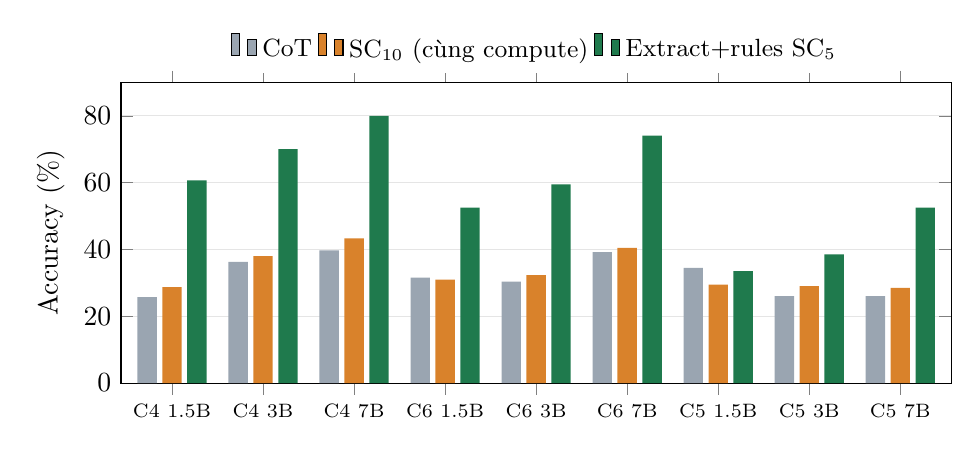
\begin{tikzpicture}
\begin{axis}[ybar, width=\linewidth, height=5.4cm, bar width=7pt, ymin=0, ymax=90,
  symbolic x coords={C4 1.5B,C4 3B,C4 7B,C6 1.5B,C6 3B,C6 7B,C5 1.5B,C5 3B,C5 7B}, xtick=data,
  x tick label style={font=\scriptsize},
  ylabel={Accuracy (\%)}, legend style={at={(0.5,1.03)},anchor=south,legend columns=3,font=\small,draw=none},
  enlarge x limits=0.07, ymajorgrids, grid style={black!10}]
\addplot[fill=xam,draw=none] coordinates {(C4 1.5B,25.7)(C4 3B,36.3)(C4 7B,39.7)(C6 1.5B,31.6)(C6 3B,30.4)(C6 7B,39.2)(C5 1.5B,34.5)(C5 3B,26.0)(C5 7B,26.0)};
\addplot[fill=mau2,draw=none] coordinates {(C4 1.5B,28.7)(C4 3B,38.0)(C4 7B,43.3)(C6 1.5B,31.0)(C6 3B,32.3)(C6 7B,40.5)(C5 1.5B,29.5)(C5 3B,29.0)(C5 7B,28.5)};
\addplot[fill=mau3,draw=none] coordinates {(C4 1.5B,60.7)(C4 3B,70.0)(C4 7B,80.0)(C6 1.5B,52.5)(C6 3B,59.5)(C6 7B,74.1)(C5 1.5B,33.5)(C5 3B,38.5)(C5 7B,52.5)};
\legend{CoT, SC$_{10}$ (cùng compute), Extract+rules SC$_5$}
\end{axis}
\end{tikzpicture}
\caption{D2: Extract+rules so với các baseline. C4: validation $k=2$--4; C6: task chưa thấy
$k=2$--4; C5: task chưa thấy $k=5$--8.}
\label{fig:d2}
\end{figure}

\begin{cachdoc}
\begin{itemize}[leftmargin=*,itemsep=1pt]
\item Trên chuỗi ngắn, mức tăng rất lớn và ổn định ở mọi kích thước: accuracy gần như gấp đôi.
  Ngay cả bản greedy (không SC) đã vượt SC$_{10}$ rất xa.
\item ``Task chưa thấy'' là một biến thể CLUTRR không hề dùng trong lúc phát triển phương pháp, nên
  kết quả không phải do ``chỉnh tay'' trên dữ liệu test.
\item Trên chuỗi dài ($k=5$--8), mức tăng tỷ lệ với kích thước mô hình: 1.5B không tăng, 3B tăng
  $+9.5$, 7B tăng $+24.0$. Kiểm định chính đăng ký trước (7B, C5) đạt
  \textcolor{luc}{\textbf{GO}}.
\item 1.5B thất bại trên chuỗi dài vì nó \emph{trích sót fact}: chỉ cần thiếu một cạnh là BFS không
  tìm được đường đi, và phương pháp rơi về CoT. Recall của bước trích fact giảm theo số bước.
\end{itemize}
\end{cachdoc}

% ----------------------------------------------------------------------------------
\subsection{D3: ablation nhân quả, mức tăng đến từ đâu?}

\paragraph{Câu hỏi.} Có hai cách giải thích cho kết quả D2: (i) việc ``trích fact'' giúp mô hình
sắp xếp thông tin rõ ràng hơn, hoặc (ii) bảng luật làm được phép hợp thành mà mô hình không làm
được. Chỉ (ii) khớp với chẩn đoán R3.

\paragraph{Thiết kế.} Giữ \emph{nguyên} các fact mà mô hình đã trích (cùng một lần sinh greedy).
Chỉ đổi \emph{bên làm phép hợp thành}:
\begin{itemize}[leftmargin=*,itemsep=1pt]
\item \textbf{LLM hợp thành}: đưa các fact đó (kèm giới tính) lại cho chính mô hình và hỏi đáp án.
\item \textbf{Luật hợp thành}: bảng luật làm như D2 (bản greedy, không SC, để so công bằng).
\end{itemize}

\begin{thietke}
Đây là một can thiệp đơn lẻ lên đúng một thành phần của pipeline: input (các fact) giống hệt nhau,
chỉ ``cơ chế'' tính đáp án khác nhau. Nếu (i) đúng, LLM hợp thành cũng phải tăng mạnh so với CoT.
Nếu (ii) đúng, LLM hợp thành $\approx$ CoT, còn bảng luật tăng mạnh.
\end{thietke}

\begin{table}[h]
\centering\small
\caption{D3: ablation trên task chưa thấy (accuracy \%, 95\% CI paired bootstrap).}
\label{tab:d3}
\begin{tabular}{llrcccc}
\toprule
Chuỗi & Mô hình & $n$ & CoT & LLM hợp thành & Luật hợp thành & Luật $-$ LLM \\
\midrule
$k=2$--4 & 1.5B & 158 & 31.6 & 32.9 & 46.2 & $+13.3$ \ci{5.1}{22.2} \\
         & 3B   & 158 & 30.4 & 28.5 & 54.4 & $+25.9$ \ci{18.4}{34.2} \\
         & 7B   & 158 & 39.2 & 36.1 & 71.5 & $+35.4$ \ci{27.2}{44.3} \\
\midrule
$k=5$--8 & 1.5B & 200 & 34.5 & 29.0 & 33.0 & $+4.0$ \ci{-3.5}{11.5} \\
         & 3B   & 200 & 26.0 & 27.0 & 32.0 & $+5.0$ \ci{-2.0}{12.5} \\
         & 7B   & 200 & 26.0 & 33.0 & 46.0 & $+13.0$ \ci{5.0}{21.0} \\
\bottomrule
\end{tabular}
\end{table}

\begin{figure}[h]
\centering
\begin{tikzpicture}
\begin{axis}[ybar, width=0.95\linewidth, height=5cm, bar width=9pt, ymin=0, ymax=80,
  symbolic x coords={ngắn 1.5B,ngắn 3B,ngắn 7B,dài 1.5B,dài 3B,dài 7B}, xtick=data,
  x tick label style={font=\small},
  ylabel={Accuracy (\%)}, legend style={at={(0.5,1.03)},anchor=south,legend columns=3,font=\small,draw=none},
  nodes near coords, every node near coord/.append style={font=\tiny}, enlarge x limits=0.1,
  ymajorgrids, grid style={black!10}]
\addplot[fill=xam,draw=none] coordinates {(ngắn 1.5B,31.6)(ngắn 3B,30.4)(ngắn 7B,39.2)(dài 1.5B,34.5)(dài 3B,26.0)(dài 7B,26.0)};
\addplot[fill=mau2,draw=none] coordinates {(ngắn 1.5B,32.9)(ngắn 3B,28.5)(ngắn 7B,36.1)(dài 1.5B,29.0)(dài 3B,27.0)(dài 7B,33.0)};
\addplot[fill=mau3,draw=none] coordinates {(ngắn 1.5B,46.2)(ngắn 3B,54.4)(ngắn 7B,71.5)(dài 1.5B,33.0)(dài 3B,32.0)(dài 7B,46.0)};
\legend{CoT, LLM hợp thành (cùng fact), Luật hợp thành (cùng fact)}
\end{axis}
\end{tikzpicture}
\caption{D3: cùng một bộ fact, chỉ đổi bên hợp thành.}
\label{fig:d3}
\end{figure}

\begin{cachdoc}
\begin{itemize}[leftmargin=*,itemsep=1pt]
\item Được đưa đúng các fact mình vừa viết ra, LLM vẫn chỉ $\approx$ CoT ($-3$ đến $+1$ điểm trên
  chuỗi ngắn). Có đủ thông tin mà vẫn không hợp thành được.
\item Bảng luật trên \emph{cùng} các fact đó cao hơn 13--35 điểm trên chuỗi ngắn ở mọi kích thước,
  và 13 điểm trên chuỗi dài ở 7B. Mức tăng tăng theo kích thước mô hình, vì mô hình lớn trích fact
  đầy đủ hơn.
\item Trên chuỗi dài, 1.5B và 3B không có khác biệt có ý nghĩa, vì khi fact bị trích thiếu thì cả
  hai bên hợp thành đều không có đủ input.
\end{itemize}
\end{cachdoc}

\begin{ketluan}
Mức tăng của D2 đến từ bước hợp thành, không phải từ bước trích fact. Đây là bằng chứng can thiệp
khép vòng với R3: R3 chẩn đoán ``đọc được nhưng không hợp thành được'', và D3 xác nhận điều đó bằng
một can thiệp thay đúng bộ phận bị hỏng.
\end{ketluan}

% ==================================================================================
\section{Những chỗ đã tự sửa trong quá trình làm}

Mỗi lỗi dưới đây được ghi trong \texttt{REVIEW.md} và đã được sửa trong paper.

\begin{table}[h]
\centering\small
\begin{tabularx}{\linewidth}{@{}>{\raggedright\arraybackslash}X>{\raggedright\arraybackslash}X>{\raggedright\arraybackslash}X@{}}
\toprule
Claim cũ & Vấn đề & Đã sửa thành \\
\midrule
Distractor làm CoT mất khoảng 10 điểm & Pilot 120 câu bị thổi phồng (winner's curse) & $n=500$: 3--6 điểm \\
``CoT dễ tổn thương hơn Direct'' & Chênh lệch không có ý nghĩa thống kê & Bỏ claim \\
Hiệu ứng CLUTRR ở 3B ``bằng placebo'' & So nhầm với placebo của vị trí khác & 7.3 \ci{3.8}{11.0}: nhỏ nhưng có thật \\
Calibration là đóng góp phương pháp & Calibration $\approx$ sinh đáp án tự do & Chỉ là baseline \\
7B MuSiQue: chọn bước cuối giúp & Do định dạng đáp án, không do suy luận & Loại \\
Attention top-4 trên 1.5B & Bug fp16 tràn số & Sửa, chạy lại; loại số liệu 7B \\
Extract (không giới tính) $+6$--8 điểm & Post hoc; xác nhận trên test $k=5$--10 thất bại & Chỉ báo cáo bản đăng ký trước \\
Giả định mixture reader của HGCD & Dữ liệu không ủng hộ & Ghi rõ trong appendix là bị bác bỏ \\
\bottomrule
\end{tabularx}
\end{table}

% ==================================================================================
\section{Tổng kết: chứng minh được gì, chưa chứng minh được gì}

\paragraph{Chứng minh được (bằng chứng mạnh, nhiều kích thước, có control).}
\begin{enumerate}[leftmargin=*,itemsep=1pt]
\item Hai cách đo ``step importance'' phổ biến (xoá một bước; resampling với baseline cố định) bị
  lệch có hệ thống. Độ lệch có công thức đóng và được xác nhận thực nghiệm (R1, R2).
\item Mô hình 0.5B--7B \emph{đọc} chuỗi chứ không \emph{suy luận qua} chuỗi; mô hình $\le$3B chép cả
  đáp án sai mà nó tự giải được (R3).
\item Tác hại của distractor lên CoT đi qua chuỗi được sinh lại (R4), nên decoding ở bước đọc đáp án
  không sửa được (R5).
\item Khi phép hợp thành được thực thi ngoài mô hình, accuracy tăng rất lớn; ablation cho thấy bước
  hợp thành là nguyên nhân (D2, D3).
\end{enumerate}

\paragraph{Chưa chứng minh được hoặc không đạt.}
\begin{itemize}[leftmargin=*,itemsep=1pt]
\item Một \emph{phương pháp decoding token} mới vượt self-consistency: HGCD, CAD, calibration và lọc
  bằng attention đều không đạt.
\item Extract+rules mới đúng trên miền có luật đóng (CLUTRR); chưa chuyển sang MuSiQue.
\item Mô hình lớn hơn 7B (Qwen2.5-14B, OLMo-2) chưa được chạy.
\end{itemize}

\section{Hạn chế}

\begin{itemize}[leftmargin=*,itemsep=1pt]
\item \textbf{Bảng luật dùng tri thức từ tập train} mà CoT không được thấy. Cần thêm baseline đưa
  bảng luật vào prompt (rules-in-prompt) hoặc program-of-thought.
\item \textbf{Extract+rules gần với Faithful CoT / Logic-LM} (hướng neuro-symbolic). Đóng góp mới
  nằm ở chẩn đoán và ablation nối chẩn đoán với can thiệp, không nằm ở bản thân pipeline.
\item \textbf{Cỡ mẫu}: mỗi ô 158--300 câu, một seed; $T_{\text{copy-wrong}}$ chỉ có 24--44 câu PS
  $=1$ mỗi mô hình.
\item \textbf{DRG dựa trên string match} nên có thể thiếu cạnh: chỉ 25\% / 36\% chuỗi liên thông,
  hop fidelity 0.57 / 0.60.
\item \textbf{Control dựa trên mask} chưa hoàn toàn trơ ở 0.5B (marker-tree AUC 0.95 trên CLUTRR+copy).
\item \textbf{Phạm vi}: chỉ hai miền (quan hệ gia đình, QA trên Wikipedia); không kết luận gì về math
  hay code.
\end{itemize}

\section{Bước tiếp theo đề xuất}

\begin{enumerate}[leftmargin=*,itemsep=1pt]
\item \textbf{Baseline công bằng hơn} cho CLUTRR: đưa bảng luật vào prompt, so với Extract+rules.
\item \textbf{Constrained decoding theo bảng luật}: mô hình vẫn tự viết CoT, nhưng token quan hệ ở mỗi
  bước hợp thành bị ràng buộc theo bảng luật. Đây là phiên bản ``decoding đúng nghĩa'' của D2, và
  tận dụng đúng phát hiện R3: sửa được chuỗi thì đáp án đúng theo.
\item \textbf{Tăng recall trích fact} cho chuỗi dài: trích theo từng câu, hoặc hợp nhất fact từ nhiều
  mẫu trước khi dựng đồ thị.
\item \textbf{MuSiQue}: tách câu hỏi thành sub-question, trả lời từng hop rồi thế bridge entity vào
  hop sau. Đây là dạng ``luật'' duy nhất có trong miền mở.
\item \textbf{Scale}: Qwen2.5-14B và OLMo-2-7B trên A100 (khoảng 1 ngày).
\end{enumerate}

\appendix
\section{Tìm file trên git}

Repo \texttt{mariorenger/DA}, nhánh \texttt{claude/funny-cori-rt5wrv}.

\begin{table}[h]
\centering\small
\begin{tabularx}{\linewidth}{@{}l>{\raggedright\arraybackslash}X@{}}
\toprule
Nội dung & Đường dẫn \\
\midrule
Báo cáo này & \texttt{paper/baocao\_vi.tex}, \texttt{paper/baocao\_vi.pdf} \\
Paper tiếng Anh & \texttt{paper/main.tex}, \texttt{paper/main.pdf} \\
Khảo sát literature về decoding & \texttt{reports/Giải mã nhân quả đa bước.md} \\
Nhật ký giả thuyết và go/no-go & \texttt{REVIEW.md} \\
Số liệu R1--R3 & \texttt{results/reliance\_v2/} \\
Số liệu R4 & \texttt{results/mediation\_n500/} \\
Số liệu R5 & \texttt{results/decoding/} \\
Số liệu D1--D3 & \texttt{results/causaldec/} (C4, C5, C6: CLUTRR; C7\_ablate: ablation;
  M\_select*, M2, M3: MuSiQue) \\
Code & \texttt{hgcd/} (round 9: \texttt{hgcd/causaldec.py}) \\
Notebook Kaggle & \texttt{notebooks/} \\
Script dựng bảng & \texttt{tools/} \\
\bottomrule
\end{tabularx}
\end{table}

\end{document}
